
Les figures ci-dessous représentent le même cube d'arête 10~cm.\\
Pour chacune des figures ci-dessous, détermine la nature des triangles surlignés.
{\em Dans chacun des cas où ils interviennent, $I$ et $J$ sont les milieux des segments sur lesquels ils se trouvent.}\\
\begin{center}
 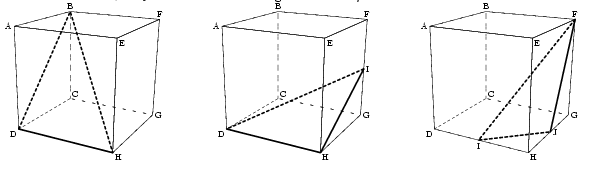
\includegraphics[scale=1]{RepS-exo2.png}
 \end{center} 

